\documentclass[a4paper, 12pt]{article}
\usepackage[utf8]{inputenc}
\usepackage[warn]{mathtext}
\usepackage[russian]{babel}
\usepackage[T2]{fontenc}
\usepackage[warn]{mathtext}
\usepackage[justification=centering]{caption}

\usepackage{graphicx}
\graphicspath{ {images/} }
\usepackage{tikz}
\usepackage{pgfplots}

\usepackage{amsmath}
\usepackage{floatflt}
\usepackage[left=20mm, top=20mm, right=20mm, bottom=20mm, footskip=10mm]{geometry}

\usepackage{multicol}
\usepackage{multirow}
\setlength{\columnsep}{2cm}

\usepackage{multicol}
\setlength{\columnsep}{2cm}
\usepackage{hyperref}
\usepackage{wrapfig}

\begin{document}
	
\begin{titlepage}
	\centering
	\vspace{5cm}
	{\scshape\LARGE Московский физико-технический институт \par}
	\vspace{4cm}
	{\scshape\Large Лабораторная работа 5.1.2 \par}
	\vspace{1cm}
	{\huge\bfseries Исследование эффекта Комптона \par}
	\vspace{1cm}
	\vfill
\begin{flushright}
	{\large выполнил студент 924 группы ФОПФ}\par
	\vspace{0.3cm}
	{\LARGE Панферов Андрей}
\end{flushright}
	

	\vfill

% Bottom of the page
	Долгопрудный, 2021 г.
\end{titlepage}

\paragraph*{Цель работы:} с помощью сцинтилляционного спектрометра исследуется энергетический спектр $\gamma$-квантов, рассеянных на графите. Определяется энергия рассеянных $\gamma$-квантов в зависимости от угла рассеяния, а также энергия покоя частиц, на которых происходит комптоновское рассеяние.


\section*{Теоретическая часть}
	Эффект Комптона -- увеличение длины волны рассеянного излучения по сравнению с падающим -- интерпретируется как результат упругого соударения двух частиц: $\gamma$-кванта и свободного электрона.
	
	Из закона сохранения 4-имульса для системы <<фотон + электрон>> следует формула для изменения длины волны рассеянного излучения:
	\begin{equation}
		\label{Kompton}
		\tag{$\star$}
		\Delta \lambda = \Lambda_K(1-\cos\theta),
	\end{equation}
	где величина $\Lambda_K = h/(mc) = 2,42 \cdot 10^{-10}$ см называется комптоновской длиной волны электрона.
	
	Из формулы (\ref{Kompton}) следует, что комптоновское смещение не зависит ни от длины волны первичного излучения, ни от рода вещества, в котором наблюдается рассеяние. В общем случае комптоновоское рассеяние происходит на свободных электронах в атоме. Для $\gamma$-квантов с энергией в несколько десятков, а тем более сотен килоэлектрон-вольт, связь электронов в атоме мало существенна, так как энергрия их связи в легких атомах не превосходит нескольких килоэлектрон-вольт, а для большинства электронов еще меньше.
	
	При рассеянии на связанных электронах изменение импульса кванта воспринимается атомом в целом. Посколько масса атома очень велика, переда ча импульса не спровождается сколь-нибудь заметной передачей энергии, и наблюдается несмещенная (по энергии) компонента в спектре рассеянного излучения. Таким образом, рассеяние $\gamma$-квантов на связанных электронах можно рассматривать как упругое столкновение квантов с атомами.
	
	Основной целью данной работы является проверка соотношения (\ref{Kompton}). Применительно к условиям нашего опыта формулу (\ref{Kompton}) следует преобразовать от длин волн к энергиям $\gamma$-квантов. Как нетрудно показать, соответсвующиее выражение имеет вид:
	\begin{equation}
		\label{1-cos}
		\tag{$\star\star$}
		\frac{1}{\varepsilon(\theta)} - \frac{1}{\varepsilon_0} = 1 - \cos \theta.
	\end{equation}

	Здесь $\varepsilon_0 = E_0/(mc^2)$ -- выраженная в единицах $(mc^2)$ энергия $\gamma$-квантов, падающих на рассеиватель, $\varepsilon(\theta)$ -- выраженная в тех же единицах энергия квантов, испытавших комптоновское рассеяние на угол $\theta$, $m$ -- масса электрона.
	
	Заменим в формуле~(\ref{1-cos}) энергию квантов, испытавших комптоновское рассеяние на угол $\theta$, номером канала $N(\theta)$, соответствующего вершине фотопика при указанном угле $\theta$:
	\begin{equation}
		\label{kek}
		\tag{$\star \star \star$}
		\frac{1}{N(\theta)} - \frac{1}{N(0)} = A (1- \cos \theta),
	\end{equation}
	где $A$ -- неизвестный коэффциицент пропорциональности между $\varepsilon(\theta)$ и $N(\theta)$.

\section*{Экспериментальная установка}
	Источником излучения служит $^{137}$Cs, испускающий $\gamma$-лучи с энергией 662 кэВ. Он помещен в толстенный свинцовый контейнер с коллиматором. Сформированный коллиматором узкий пучок $\gamma$-квантов попадает на графитовую мишень 2 (цилиндр диаметром 40 мм и высотой 100 мм.)
	
	\begin{figure}[h!]
	    \centering
		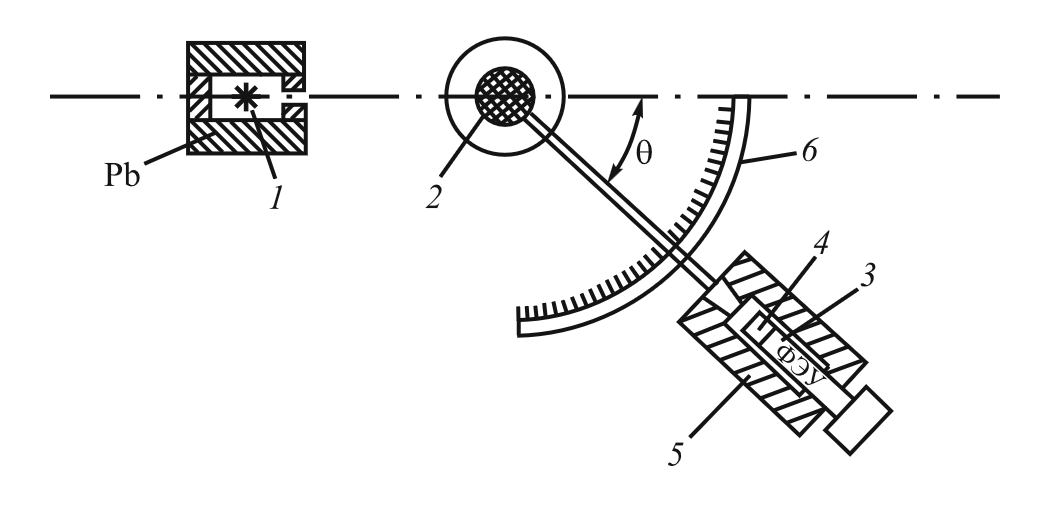
\includegraphics[width=14cm]{ust.png}
		\caption{Экспериментальная установка.}
		\label{fig:ust}
	\end{figure}
	
	Кванты, испытавшие комптоновское рассеяние в мишени, регистрируются сцинтилляционным счетчиком. Счетчик состоит из фотоэлектронного умножителя 3 (далее ФЭУ) и сцинтиллятора 4. Сцинтиллятором служит кристалл NaI(Tl) цилиндрической формы диаметром 40 мм и высотой 40 мм, его выходное окно находится в оптическом контакте с фотокатодом ФЭУ. Сигналы, возникающие на ФЭУ, подаются на ЭВМ для амплитудного анализа. Кристалл и ФЭУ расположены в светонепроницаемом блоке, укрепленном на горизонтальной штанге. Штанга вместе с этим блоком может вращаться относительно мишени, угол поворота отсчитывается по лимбу 6.
	
	На Рис.~\ref{fig:ust} представлена функциональная блок-схема измерительного комплекса, который состоит из ФЭУ, питаемого от высоковольтного выпрямителя ВСВ, обеспечивающего работу ФЭУ в спектрометрическом режиме, усилителя-анализатора УА, являющегося входным интерфейсом ЭВМ, управляемой с клавиатуры КЛ. В ходе проведения эксперимента информация отражается на экране дисплея Д, окончательные результаты в виде таблиц и графиков могут быть выведены на принтер ПР.
	
	\section*{Экспериментальные данные}
	
		\begin{table}[h]
			\caption{Измеряемые величины и их погрешность.}
			\centering
			\label{table:parametr}
			\begin{tabular}{|c|c|c|c|}
				\hline
				$\theta$, $^\circ$ & $\sigma_\theta$, $^\circ$ & $N$ & $\sigma_N$ \\ \hline
				0,0                & \multirow{11}{*}{0,5}     & 790 & 20         \\ \cline{1-1} \cline{3-4} 
				10,0               &                           & 770 & 10         \\ \cline{1-1} \cline{3-4} 
				20,0               &                           & 680 & 30         \\ \cline{1-1} \cline{3-4} 
				30,0               &                           & 630 & 20         \\ \cline{1-1} \cline{3-4} 
				40,0               &                           & 590 & 40         \\ \cline{1-1} \cline{3-4} 
				50,0               &                           & 530 & 40         \\ \cline{1-1} \cline{3-4} 
				60,0               &                           & 440 & 50         \\ \cline{1-1} \cline{3-4} 
				70,0               &                           & 400 & 50         \\ \cline{1-1} \cline{3-4} 
				80,0               &                           & 350 & 40         \\ \cline{1-1} \cline{3-4} 
				90,0               &                           & 320 & 50         \\ \cline{1-1} \cline{3-4} 
				100,0              &                           & 300 & 50         \\ \hline
			\end{tabular}
		\end{table}
	
	
%		\begin{table}[h]
%			\caption{Счетная характеристика ФЭУ № 4012.}
%			\centering
%			\label{table:schet}
%			\begin{tabular}{|c|c|c|c|c|}
%				\hline
%				$t$, с              & $U$, кВ & $\sigma_U$, кВ       & Счет  & $\sigma_\text{Счет}$   \\ \hline
				%\multirow{7}{*}{60} & 1,2     & \multirow{7}{*}{0,5} & 16000 & \multirow{7}{*}{2000} \\ \cline{2-2} %\cline{4-4}
				%& 1,3     &                      & 51000 &                       \\ \cline{2-2} \cline{4-4}
				%& 1,4     &                      & 63000 &                       \\ \cline{2-2} \cline{4-4}
				%& 1,5     &                      & 63000 &                       \\ \cline{2-2} \cline{4-4}
				%& 1,6     &                      & 71000 &                       \\ \cline{2-2} \cline{4-4}
				%& 1,7     &                      & 69000 &                       \\ \cline{2-2} \cline{4-4}
				%& 1,8     &                      & 71000 &                       \\ \hline
			%\end{tabular}
		%\end{table}
	

		
	\section*{Обработка результатов}
		Оценим погрешности величин $1 - \cos \theta$ и $1/N$ по следующим формулам:
		\begin{equation*}
			\sigma_{1-\cos \theta} = \sin \theta \cdot \sigma_\theta, \ \sigma_{1/N} = 1/N^2 \cdot \sigma_N.
		\end{equation*}
			
		Результаты вычислений представлены в Таблице \ref{table:data}:
		
		Изобразим экспериментальные результаты (табл.~\ref{table:data}) в виде графика (рис.~\ref{graph:angular}). Согласно формуле (\ref{kek}) экспериментальные точки должны лежать на одной прямой, что, как видно, выполняется. Пересечение этой прямой с осью ординат определяет наилучшее значение $N(0)$, а пересечение линии $1 - \cos \theta = 1$ позволяет найти наилучшее значение $N(90)$. 
		
        \vspace{0.5cm}
        \begin{minipage}{0.5\textwidth}
            \centering
			\captionof{table}{Обработанные данные.}
			\label{table:data}
			\begin{tabular}{|c|c|c|c|}
				\hline
				$1 - \cos \theta$ & $\sigma_{1-\cos \theta}$ & $1/N \cdot 10^3$ & $\sigma_{1/N}$ \\ \hline
				0,000             & 0                        & 1,27  & 0,02           \\ \hline
				0,015             & 0,002                    & 1,30  & 0,02           \\ \hline
				0,060             & 0,003                    & 1,48  & 0,05           \\ \hline
				0,134             & 0,004                    & 1,58  & 0,04           \\ \hline
				0,234             & 0,006                    & 1,7   & 0,1            \\ \hline
				0,357             & 0,007                    & 1,9   & 0,1            \\ \hline
				0,500             & 0,008                    & 2,3   & 0,2            \\ \hline
				0,658             & 0,008                    & 2,5   & 0,3            \\ \hline
				0,826             & 0,009                    & 2,9   & 0,3            \\ \hline
				1,000             & 0,009                    & 3,1   & 0,4            \\ \hline
				1,174             & 0,009                    & 3,4   & 0,6            \\ \hline
			\end{tabular}
        \end{minipage}
        \begin{minipage}{0.5\textwidth}
            \begin{tikzpicture}[scale=1]
                \centering
                \label{graph:angular}
                \begin{axis}[
                    	axis lines = middle,
                    	xlabel = {$1 - cos(\theta)$},
                        ylabel = {$N\cdot10^3$},
                    	ylabel style={red, scale=1},
                        xlabel style={red, scale=1},
                        title style={align=left}, title={Связь номера канала пика с углом},
                    	table/col sep=semicolon,
                    ]
            	    \addplot +[blue, only marks, error bars/.cd,x dir=both, x explicit,y dir=both, y explicit] table[x=A, y=iN, x error=sA, y error=siN]{hits.txt};
            	    \addplot[color=red, domain=0:1.2]{1.82 * x + 1.33};
            	\end{axis}
            \end{tikzpicture}
        \end{minipage}
        \vspace{0.5cm}

\section*{Обсуждение результатов и выводы}
	Итак, в настоящей лабораторной работе нами была проведена проверка соотношения (\ref{Kompton}). Экспериментально установлено, что $\gamma$-кванты действительно испытывают упругое рассеяние на свободных частицах. 
	
	Обратим наше внимание на то, что с увеличением угла $\theta$ погрешность измерения номера канала $\sigma_N$ увеличивается, что связано со смещением фотопика в сторону сплошного распределения, обязанного комптоновскому рассеянию. При $\theta = 110^\circ$ уже было невозможно увидеть пик полного поглощения.
	
	На основании таблицы \ref{table:data} можно определить энергию покоя частиц, на которых происходит комптоновское рассеивание. Путем несложных преобразований формула (\ref{1-cos}) принимает вид:
	\begin{equation*}
		mc^2 = E(0) \frac{N(90)}{N(0)-N(90)},
	\end{equation*}
	где $E(0)$ -- энергия $\gamma$-лучей, испускаемых источником (в нашем случае $^{137}$Cs), то есть 662 кэВ. Имеем:
	\[
	\boxed{mc^2 = 430 \pm 20 \ \text{кэВ}}.
	\]
	Видно, что результат на 16\% меньше 511 кэВ -- энергии покоя электрона. 

\end{document}